\documentclass[a4paper, oneside, final]{scrartcl}

\usepackage[spanish]{babel}
\usepackage{scrlayer-scrpage}
\usepackage{titlesec}
\usepackage{anysize}
\usepackage{marvosym}
\usepackage{tabularx,colortbl}
\usepackage{ebgaramond}
\usepackage{microtype}
\usepackage{bera}
\usepackage{listings}
\usepackage{xcolor}
\usepackage{hyperref}
\usepackage{graphicx}
\usepackage{amsmath}
\usepackage{cite}

\titleformat{\section}{\large\scshape\raggedright}{}{0em}{}[\titlerule]

\pagestyle{scrheadings}

\addtolength{\voffset}{-0.5in}
\addtolength{\textheight}{3cm}

\newcommand{\gray}{\rowcolor[gray]{.90}}

\renewcommand{\headfont}{\normalfont\rmfamily}

\marginsize{2cm}{2cm}{2cm}{2cm}
\setlength{\parindent}{0cm}

\colorlet{punct}{red!60!black}
\definecolor{background}{HTML}{EEEEEE}
\definecolor{delim}{RGB}{20,105,176}
\colorlet{numb}{magenta!60!black}

\lstdefinelanguage{json}{
    basicstyle=\normalfont\ttfamily,
    numbers=left,
    numberstyle=\scriptsize,
    stepnumber=1,
    numbersep=8pt,
    showstringspaces=false,
    breaklines=true,
    frame=lines,
    backgroundcolor=\color{background},
    literate=
     *{0}{{{\color{numb}0}}}{1}
      {1}{{{\color{numb}1}}}{1}
      {2}{{{\color{numb}2}}}{1}
      {3}{{{\color{numb}3}}}{1}
      {4}{{{\color{numb}4}}}{1}
      {5}{{{\color{numb}5}}}{1}
      {6}{{{\color{numb}6}}}{1}
      {7}{{{\color{numb}7}}}{1}
      {8}{{{\color{numb}8}}}{1}
      {9}{{{\color{numb}9}}}{1}
      {:}{{{\color{punct}{:}}}}{1}
      {,}{{{\color{punct}{,}}}}{1}
      {\{}{{{\color{delim}{\{}}}}{1}
      {\}}{{{\color{delim}{\}}}}}{1}
      {[}{{{\color{delim}{[}}}}{1}
      {]}{{{\color{delim}{]}}}}{1},
}

\begin{document}

\thispagestyle{empty}

\begin{center}
    %\newcommand{\HRule}{\rule{\linewidth}{0.5mm}}
    \begin{minipage}{0.29\textwidth} 
        \center{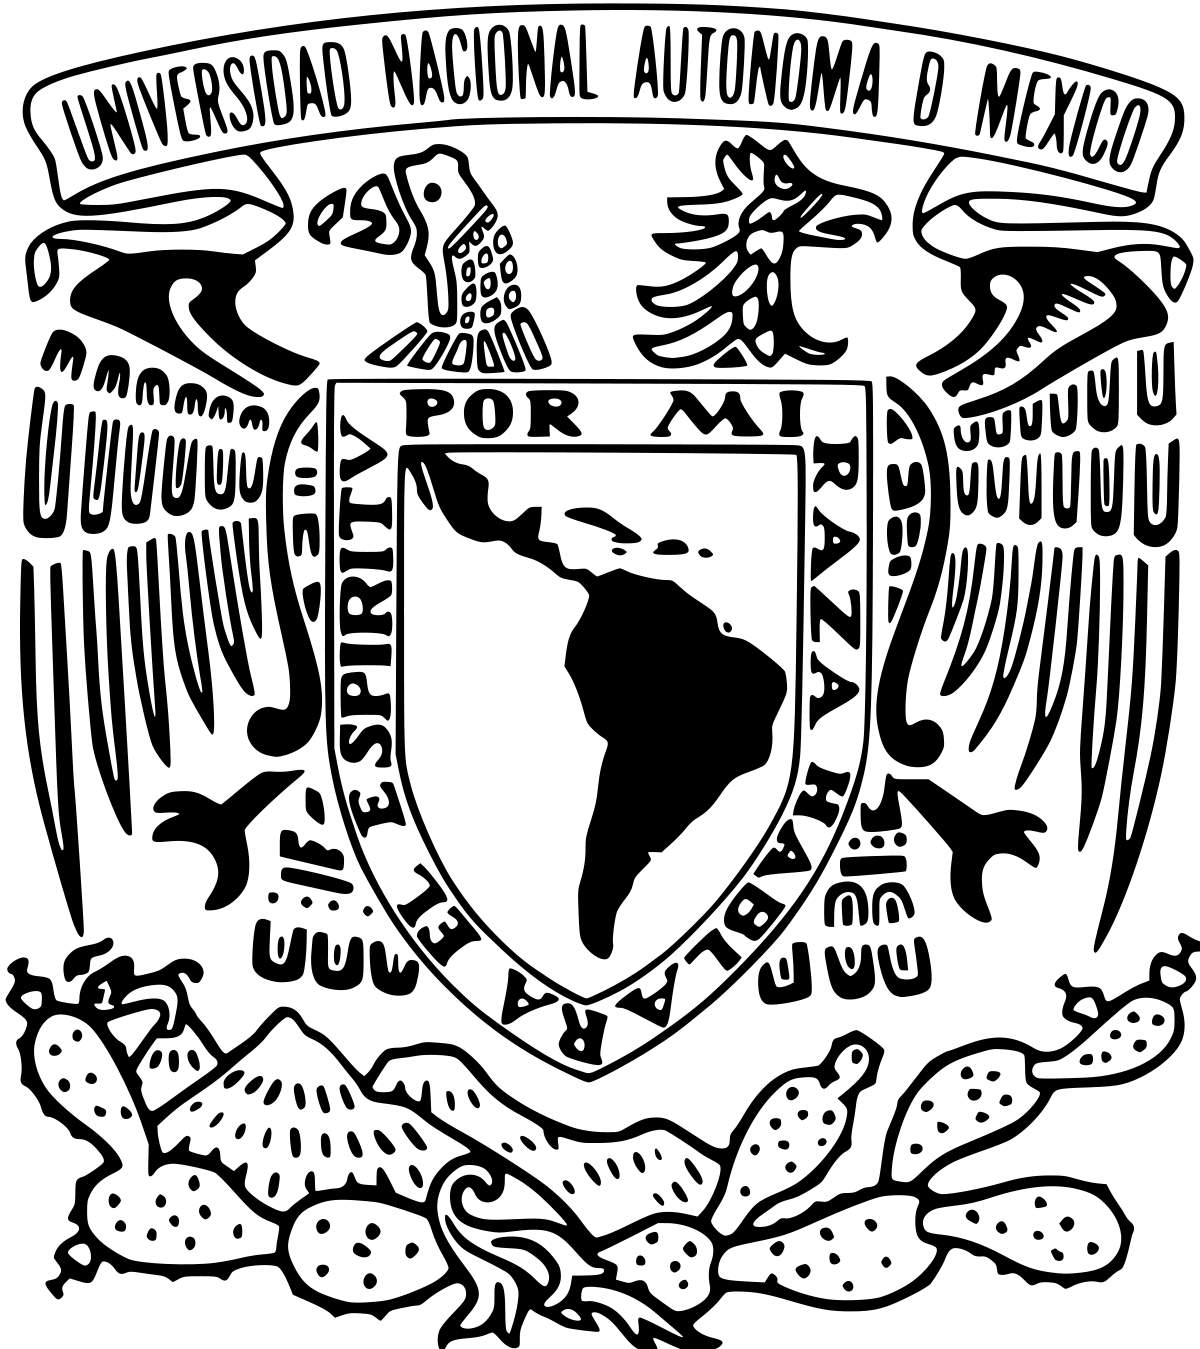
\includegraphics[scale = 0.06]{images/logo_unam.png}}
    \end{minipage}
    \begin{minipage}{0.40\textwidth} 
    \center{\textsc{\LARGE Universidad Nacional \\[5mm] Autónoma de México}}\\
    \end{minipage}
    \begin{minipage}{0.29\textwidth}
        \center{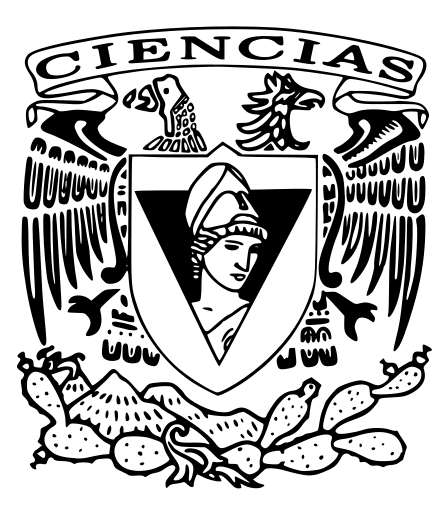
\includegraphics[scale =0.18]{images/logo_ciencias.png}}
    \end{minipage}
    \vspace{5mm}					
    
    \textsc{\noindent \LARGE Facultad de Ciencias}\\[20mm]
    
    \textsc{\LARGE   Ingeniería de Software \\[5mm]
                    \LARGE 2024-2}      \\[20mm]
    
    \textsc{\textbf{\huge   Análisis de requerimientos}}\\[5mm]
    \textsc{\LARGE  Pizarra colaborativa para computólogos}\\[20mm]

    \LARGE
    \textsc{Equipo I}\\[5mm]
    \Large 
    \textsc{Diego Sebastián Sánchez Correa}\\[2mm]
    \textsc{Mauro Emiliano Chávez Zamora}\\[2mm]
    \textsc{Ulises Josué Anaya Pérez}\\[2mm]
    \textsc{Daniel Linares Gil} \\[2mm]
    \textsc{Karyme Ivette Azpeitia García}
    \\[20mm]

    \large Creado: 15/02/2024\\[2mm]
    \large Última actualización: 20/02/2024\\
    
\end{center}	
\newpage  


\section{Objetivo}

El objetivo de este documento es diseñar una aplicación web para la creación y edición de pizarras que permita la colaboración entre usuarios en tiempo real.

\section{Contexto}

Existen múltiples aplicaciones para la edición de pizarras, como 
\href{https://miro.com/}{Miro}, \href{https://www.figma.com/figjam/}{Figjam} y \href{https://jamboard.google.com}{Jamboard}. Nuestro objetivo es desarrollar una herramienta similar que permita utilizar funcionalidades para específicas a nuestra área de conocimiento; lo cual incluye el poder crear gráficas y expresar expresiones/fórmulas matemáticas con facilidad.

\section{Herramientas elegidas}

En la sección del front-end elegimos la herramienta VUE, la cual es un \textit{framework} de JavaScript, que nos permite trabajar a través de componentes que nos den un diseño web modular, la idea es que VUE cargue los componentes de manera predeterminada para simular la navegación en la aplicación, esto se conoce como \textit{SPA (Single page application)} y nos permitiría que la aplicación se ejecutara con fluidez para generar una buena impresión en la persona usuaria.

Por otro lado, para el back-end, decidimos utiliar NestJS debido a que es uno de los frameworks m\'as populares para Javascript, adem\'as, ofrece soporte para Typescript, que, como es tambi\'en usado dentro del front-end, facilita el desarrollo conjunto (si la herramienta es compartida entre back-end y front-end, el desarrollo se torna una tarea m\'as simple) as\'i como la incorporaci\'on de bibliotecas dentro de ambas.

\section{Edición concurrente de pizarras}

Existen dos métodos principales para colaboración en tiempo real, \textit{Operational transformation} (OT) y \textit{Conflict free replicated data types} (CRDT).

\textit{Operational transformation} es el primer método que surgió para colaboración en tiempo real. Consiste en que un servidor central se encarga de aplicar los cambios a los documentos y funciona como la fuente de verdad. Cuando múltiples usuarios modifican el documento de manera concurrente, el servidor se encarga de transformar las operaciones concurrentes para que se apliquen. 

Por ejemplo, se tiene el texto inicial 'ttexto', y se realizan dos operaciones concurrentes. Alice elimina la letra en la posición 1, y de manera concurrente, Bob inserta una 'o' a la derecha de la posición 4. Si el servidor procesa la operación realizada por Alice antes que la de Bob, entonces debe modificar el índice de la inserción de Bob para que esta ocurra en la posición 3, porque al eliminarse la letra en la posición 1, las letras a su derecha se movieron una posición a la izquierda.

OT es el método más utilizado en la actualidad y lo utilizan aplicaciones como Google Docs. Sin embargo, este método tiene algunos inconvenientes. El principal inconveniente es que necesita un servidor central que funcione como fuente de verdad, por lo cual es más difícil de escalar, y se dificulta la edición de documentos sin acceso a internet.

En los últimos años se ha desarrollado un nuevo método para la edición de documentos colaborativa, conocido como \textit{Conflict free replicated data types} (CRDT). La idea principal de CRDT es que los documentos se almacenan en una estructura de datos que permite que los cambios realizados por múltiples usuarios se puedan sincronizar de manera consistente. 

La principal ventaja de los CRDT es que están diseñados para sistemas distribuidos, y no necesitan un servidor central. Cada usuario edita su copia del documento y cuando los usuarios sincronizan los cambios, existe la garantía de que todas las copias convergen al mismo estado final. Los CRDT facilitan la edición de documentos sin conexión y también permiten el intercambio de la información en esquemas P2P donde no existe un servidor central. 

La principal desventaja de los CRDT es que el tamaño del documento crece rápidamente por la información extra que almacenan. Sin embargo, en la actualidad existen implementaciones de CRDT como Yjs \cite{yjs-no-date} que realizan múltiples optimizaciones. En \cite{jahns-2020}, se muestra que Yjs puede manejar documentos de gran tamaño, con una complejidad en tiempo lineal para procesar el documento respecto al número de operaciones. Además, el espacio utilizado por Yjs para almacenar los documentos, es solamente de 1.5 a 2 veces mayor al utilizado en el documento original. Podría parecer que un aumento de 2 veces en el tamaño del documento puede incrementar significativamente el tráfico de red cuando cada vez que se abre el documento. Sin embargo, se puede almacenar una copia del documento de manera local, y que cuando se vuelva a abrir solo se transfieran las actualizaciones que se realizaron.

Se utilizará Yjs para manejar la edición concurrente de las pizarras. Yjs es uno de los protocolos de CRDT más populares y es utilizado por defecto por Blocksuite \cite{unknown-author-no-date}, la biblioteca que se utilizará para la edición de texto. 

\section{Autenticación}

La autenticación utilizará \textit{JSON web tokens} (JWT). JWT permite verificar la identidad de un usuario sin necesidad de almacenar información de la sesión en la base de datos, por lo cual es más eficiente que si fuera necsario buscar la sesión en la base de datos. Por otro lado, la principal desventaja de utilizar JWT es que no permite un control de las sesiones de usuario, una vez se genere el \textit{token JWT}, no es posible invalidar la sesión hasta que expire. Para mitigar lo anterior, los \textit{tokens} se generan con un tiempo de expiración corto (tentativamente un día). 

Se implementará una ruta en la API para registrar al usuario, y otra para iniciar sesión, las cuales se muestran a continuación.

\begin{itemize}
    \item \texttt{POST /api/auth/login}
\begin{lstlisting}[language=json,firstnumber=1]
Request:
{
    "email": "user1@mail.com",
    "password": "password"
}

Response:
STATUS: 200 OK
{
    "token": "json-web-token"
}

Response Error:
STATUS: 404 NOT FOUND
\end{lstlisting}
    
\item \texttt{POST /api/auth/register}
\begin{lstlisting}[language=json,firstnumber=1]
Request:
{
    "username": "username"
    "email": "user1@mail.com",
    "password": "password"
}

Response:
STATUS: 200 OK
{
    "token": "json-web-token"
}

Response Error:
STATUS: 404 NOT FOUND
\end{lstlisting}

\end{itemize}

\section{Autorización}
Inicialmente, antes de la introducci\'on del concepto de espacios de trabajo, parec\'ia natural asociar a los usuarios con las pizarras directamente; pero la administraci\'on de permisos de pizarras, en conjunto con aquellos definidos para los espacios de trabajo, se torn\'o una tarea compleja e innecesaria. Si las pizarras se trataban de subconjuntos de espacios de trabajo, por qu\'e lidiar con cada uno de los subconjuntos si pod\'iamos establecer a los espacios de trabajo como la unidad b\'asica de trabajo.

De esta manera, llegamos a la conclusi\'on de que la mejor opci\'on ser\'ia definir los permisos de escritura, lectura y administrador entre los usuarios y un espacio de trabajo. Estos ser\'an administrados a partir de URLs (generados por el creador del espacio de trabajo) que contendr\'an Json Web Tokens que permitir\'a asociar al usuario con el espacio de trabajo particular.

\section{Colaboración}
La aplicación debe ser capaz de compartir un enlace a las personas que el usuario desee se integren a su pizarra, utiliza el identificador de manera que se pueda designar permisos de lectura/edición. Si bien se generan permisos por defecto y otros se pueden asignar personalmente a cada usuario, también es necesario que la aplicación revise los permisos de acceso más restrictivos de manera que no caigamos en irregularidades de seguridad, el link poseerá la referencia al atributo \textit{whiteboardID} en la tabla que lleva el registro, de manera que sólo será necesario revisar el acceso cuando un usuario trate de acceder a una pizarra en concreto.

La pizarra lleva registro de las personas que tienen permitido editarla a través del JWT \textit{(Jason Web Token)}, el cual sólo identifica perfiles activos, sino que también se articula con los identificadores de la pizarra para verificar qué permisos de colaboración poseen las personas usuarias. La idea es que las modificaciones también tengan un seguimiento a través del \textit{token} de identificación.

Blocksuite será nuestra herramienta que gestionará la colaboración desde el lado del frontend a través de su integración con los componentes que muestran la pizarra en pantalla.

\section{Comentarios}

La idea es que al tener una pizarra colaborativa, muchos usuarios pueden hacer cambios de manera simultanea por esa razón , nos pareció muy útil poder incluir comentarios ya que al ser un espacio de trabajo compartido , necesitamos que exista una manera de poder comunicar a los demás colaboradores alguna observación o sugerencia sobre alguna parte del contenido en la pizarra.
Entonces tenemos algunas opciones para implementar los comentarios
\begin{itemize}
    \item \textbf{Opción back-end:}
    La primera opción que tenemos para usar comentarios en la pizarra es crear una entidad dentro de la base de datos.
    \item \textbf{Opcion blocksuite:}
    Esta opción se basa en la posibilidad de definir los comentarios de un documento como datos embebidos en el formato del documento.
\end{itemize}

\section{Servidor de WebSockets}
La naturaleza dinámica de la pizarra colaborativa
hace de los \textit{websockets} una buena opción que facilita
 la sincronización de cambios entre
 varios usuarios que trabajan en ella al mismo tiempo.

Las bases de datos comunes no son lo suficientemente r\'apidas para administrar actualizaciones en tiempo real de aplicaciones cuyo cambio sucede muy rápidamente; la pizarra colaborativa es un ejemplo ideal de este tipo de aplicaciones.

Buscando algunas bibliotecas pensamos que es una buena opción hacer uso de y-redis que es una alternativa de back-end para y-websockets .

\textit{Redis} (Remote Dictionary Server) es una base de datos multimodelo que se cre\'o a partir de la idea de que el cach\'e tambi\'en puede ser una unidad de almacenamiento no vol\'atil. Se trata de un sistema en el que la informaci\'on siempre es modificada o le\'ida de la memoria principal (RAM); esto, naturalmente, induce una latencia de milisegundos. En conjunto, escribe la informaci\'on al disco para que otorgar la capacidad de reconstrucci\'on.

Redis es usada como cach\'e y canal de distribuci\'on para actualizaciones en documentos, al tener una pizarra colaborativa , se generan much\'isimas operaciones cada momento, por lo que hace sentido usar redis-cache para almacenamiento temporal para distribuir documentos lo más rápido posible.


\section{Edición de documentos}

Para la edición de documentos se utilizará Blocksuite \cite{unknown-author-no-date}. Blocksuite es un \textit{framework} para edición de documentos moderno que incluye soporte para colaboración en tiempo real a través de Yjs. Además, Blocksuite incluye funciones de edición de texto avanzadas y soporte para dibujo sobre el canvas, lo cual lo hace muy conveniente para el desarrollo de una pizarra colaborativa. 

En Blocksuite el código se organiza en bloques, los cuales son similares a la noción de componentes en Vue. El documento se representa como un árbol de bloques a partir de un bloque raíz. Por ejemplo, la imagen debajo muestra un ejemplo de las estructura del árbol de bloques.

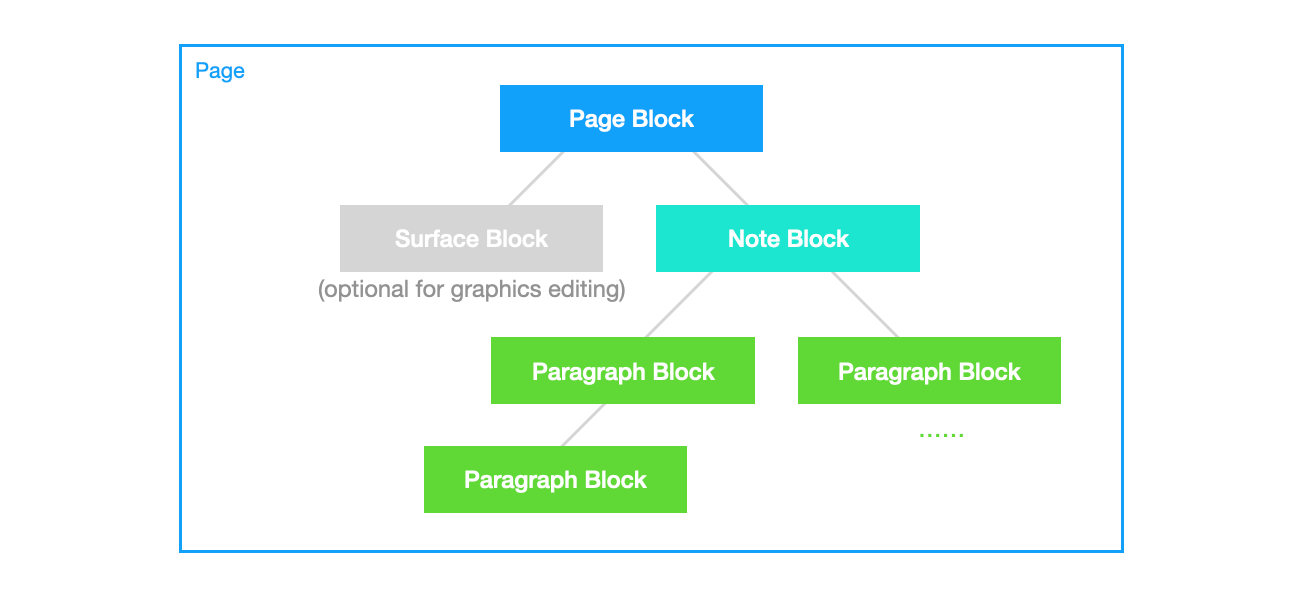
\includegraphics[width=\textwidth]{images/block-nesting.png}

Cada bloque se compone por \textit{schema},\textit{service} y \textit{view}, los cuales corresponden al modelo, controlador y vista de MVC. Además, los bloques pueden tener asociados \textit{fragments}, los cuales contienen funcionalidad que puede ser reutilizada en distintos bloques, por ejemplo, una barra de opciones flotante que aparece al seleccionar un bloque. La estructura de los bloques permite que se puedan extender de manera sencilla.

Blocksuite también provee una biblioteca de bloques que se pueden utilizar para la pizarra. Estos bloques se renderizan como componentes web, utilizando Lit. La principal razón por la cual utilizan componentes web es porque se pueden integrar en la mayoría de \textit{frameworks} (Vue tiene buen soporte), y los componentes web se renderizan directamente en el DOM, a diferencia de \textit{frameworks} como Vue, en los cuales se utiliza un DOM virtual.

Se podría implementar un renderizado de Blocksuite para Vue, pero sería necesario reimplementar al menos la vista de todos los componentes a utilizar. Por lo anterior, se utilizará Lit para implementar los bloques de Blocksuite, y Vue para todo lo demás. Los componentes que requieran interactuar con el editor pero no sean dinámicos, como por ejemplo la barra de herramientas de edición, se implementarán en Vue.

Para configurar Blocksuite dentro de la aplicación de Vue se utilizarán dos componentes. El componente \texttt{EditorProvider} será el encargado de inicializar el editor de Blocksuite, y proveerlo como estado de la aplicación utilizando \texttt{provide}. Todos los componentes que necesitan acceder al editor necesitan ser hijos del componente \texttt{EditorProvider}. El componente \textit{EditorContainer} se encarga de inyectar el componente web raíz del editor en el DOM.
\section{Entidad relación}

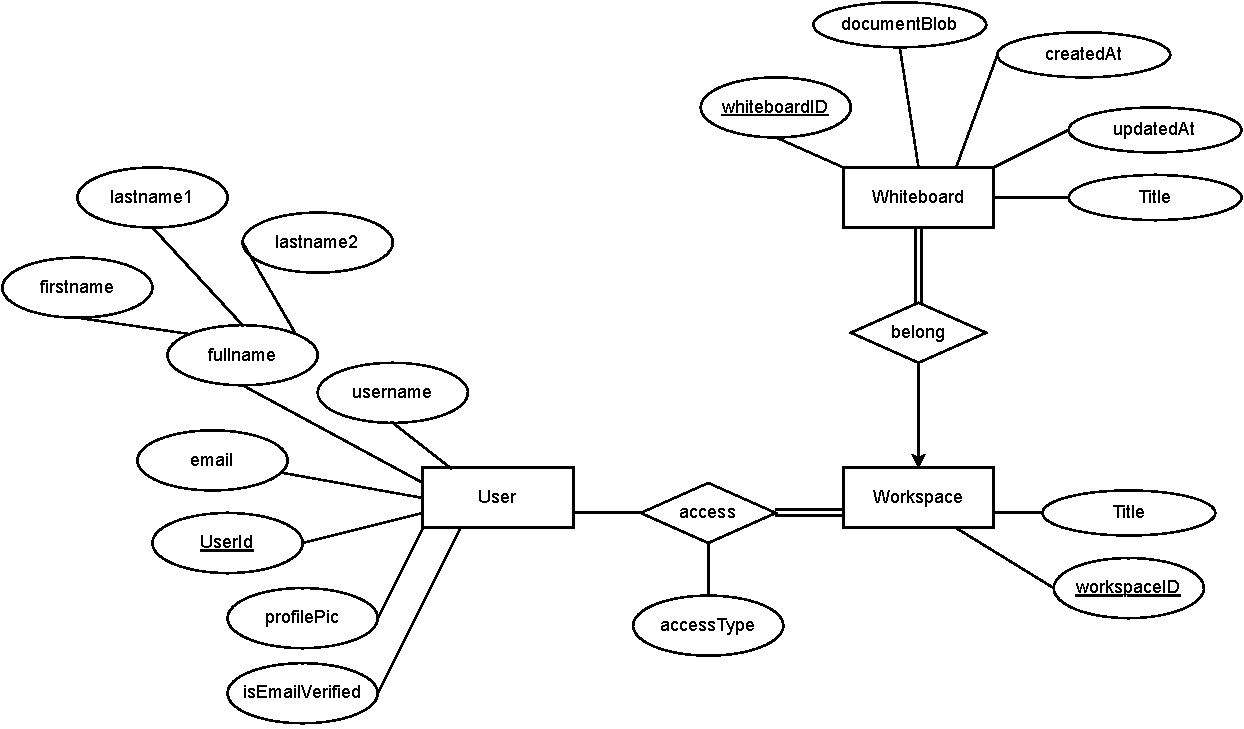
\includegraphics[width=\textwidth]{images/Entidad-relacion.pdf}

\textbf{Nota:} Inicialmente se tiene pensado almacenar el documento en formato binario como un atributo de la entidad \textit{Whiteboard}. Se iterará a partir del diseño inicial para optimizar cómo se almacena el documento.

\section{Wireframes Pizarra}
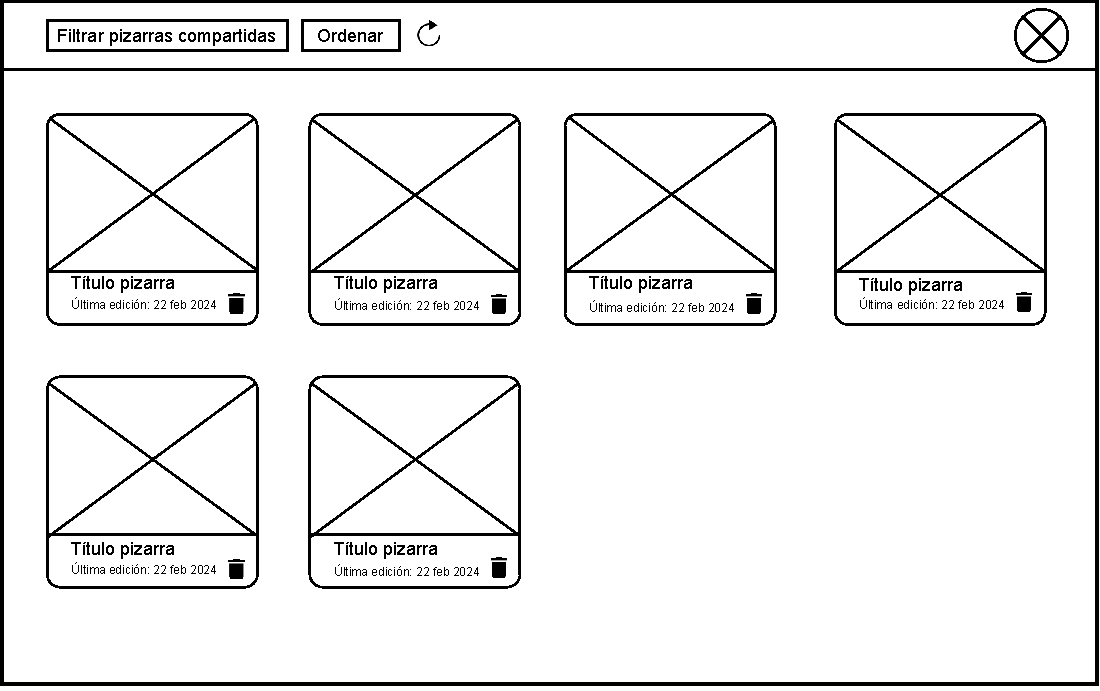
\includegraphics[width= \textwidth]{images/WireframeListaPizarras.drawio.pdf}

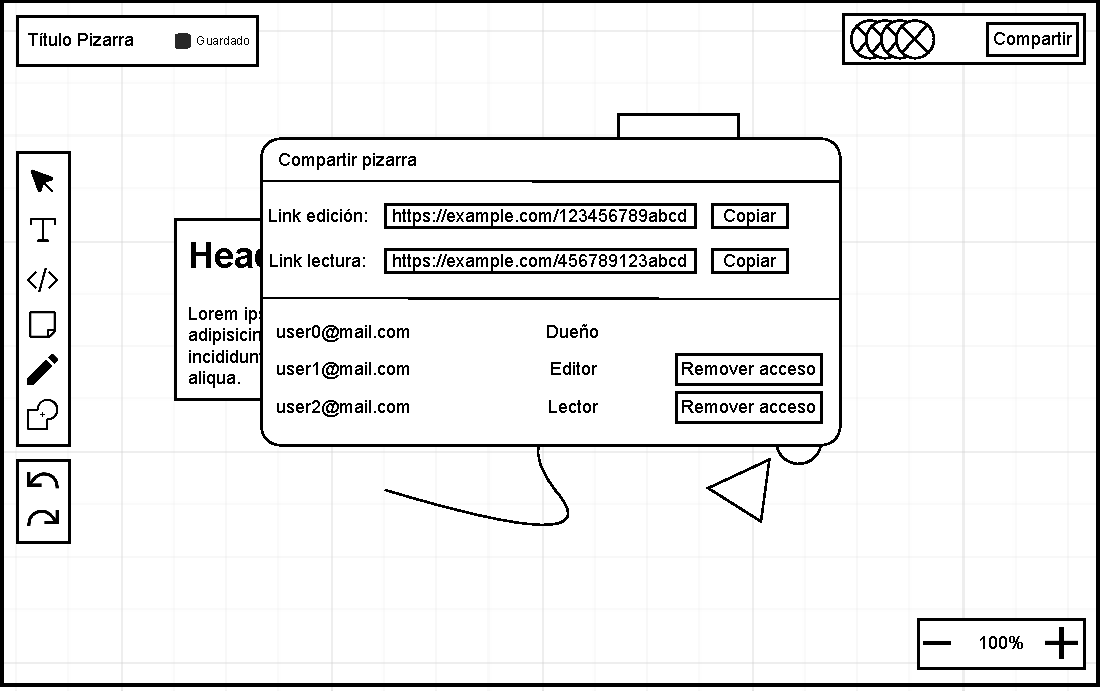
\includegraphics[width= \textwidth]{images/WireframePizarra-Ventana-compartir-pizarra.drawio.pdf}
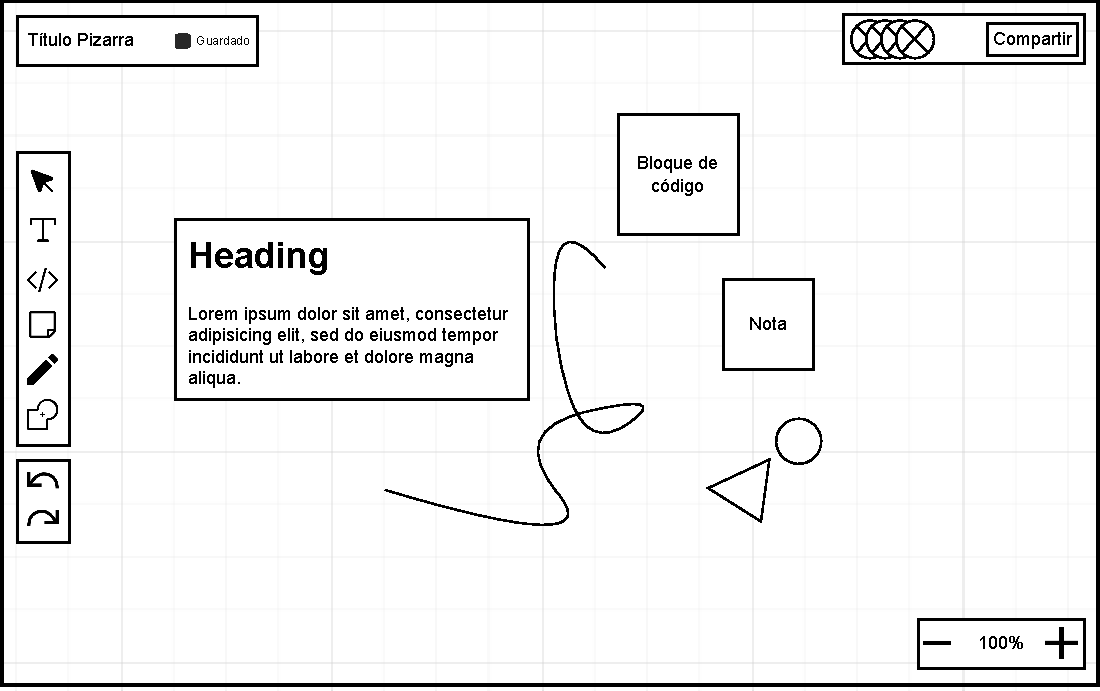
\includegraphics[width= \textwidth]{images/WireframePizarra.drawio.pdf}


\clearpage

\section{Casos de Uso}

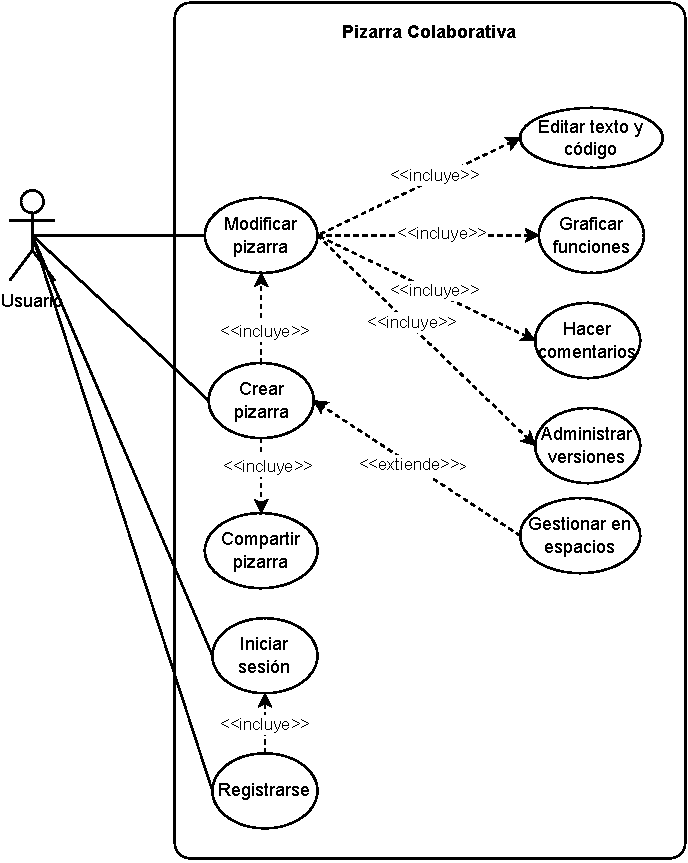
\includegraphics[width=\textwidth]{images/Casos-de-uso-1.pdf}

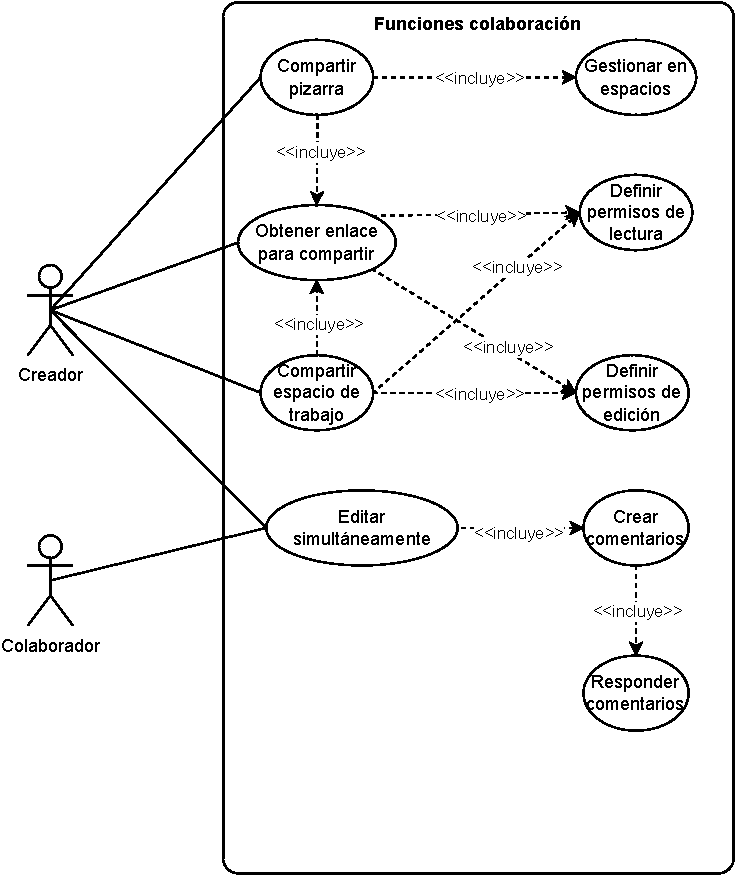
\includegraphics[width=\textwidth]{images/Casos-de-uso-2.pdf}

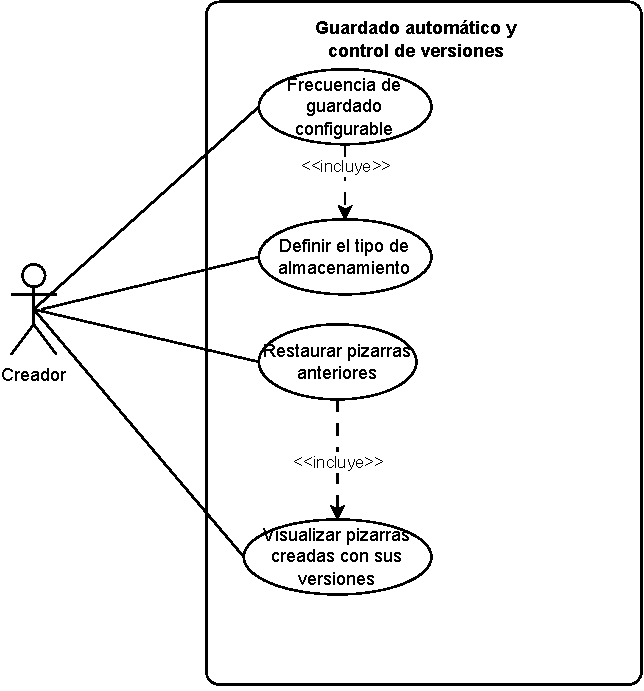
\includegraphics[width=\textwidth]{images/Casos-de-uso-3.pdf}


\bibliography{refs}{}
\bibliographystyle{plain}
\end{document}